% id: 41-09
% book: 베이직쎈 확률과 통계 · 03 확률의 뜻과 활용
% section: 유형 023 배반사건
% figure: tikz:fig-41-09
% answer: 
% answer_source: 
% variant_level: 0 (원본 전사)
% 이 파일은 build.mjs 가 items.json 에서 만든다. 고칠 때는 items.json 을 고친다.
\smash{\raisebox{1.5mm}{\dmkichul{베이직쎈 확률과 통계 41쪽 09번}}}
\noindent\begin{minipage}[t]{0.58\linewidth}\vspace{0pt}\raggedright 표본공간 $S=\{1{,}\mkern3mu\mathopen{}2{,}\mkern3mu\mathopen{}3{,}\mkern3mu\mathopen{}4{,}\mkern3mu\mathopen{}5{,}\mkern3mu\mathopen{}6\}$의 부분집합인 두 사건 $A$, $B$가 오른쪽 벤 다이어그램과 같을 때, 옳은 것만을 보기에서 있는 대로 고르시오.\end{minipage}\hfill\begin{minipage}[t]{0.4\linewidth}\vspace{0pt}\centering \resizebox{\ifdim\width>\linewidth\linewidth\else\width\fi}{!}{% 유형 023 41-09(인쇄 41쪽) — 표본공간 S 안에 사건 A 의 원, 그 안에 사건 B 의 원이 놓인 벤 다이어그램.
%   원소 자리: A 밖 1·4, A 안 B 밖 2·5, B 안 3·6. 스캔 화질이 낮아 TikZ 로 다시 그림.
% 라벨(S·A·B·원소)은 원문에 있는 것만. 라벨은 원문처럼 선을 끊고 그 자리에 놓는다.
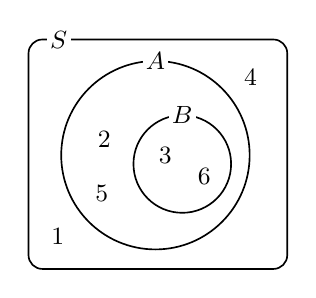
\begin{tikzpicture}[scale=0.62, line width=0.5pt]
  \draw[rounded corners=5pt, line width=0.6pt] (0,0) rectangle (5.3,4.7);
  \draw[line width=0.6pt] (2.6,2.33) circle (1.93);
  \draw[line width=0.6pt] (3.15,2.15) circle (1.0);
  \node[fill=white, inner sep=1.2pt, font=\small] at (0.62,4.7) {$S$};
  \node[fill=white, inner sep=1.2pt, font=\small] at (2.6,4.26) {$A$};
  \node[fill=white, inner sep=1.2pt, font=\small] at (3.15,3.15) {$B$};
  \node[font=\small] at (1.55,2.65) {$2$};
  \node[font=\small] at (1.50,1.55) {$5$};
  \node[font=\small] at (2.80,2.32) {$3$};
  \node[font=\small] at (3.60,1.90) {$6$};
  \node[font=\small] at (0.60,0.67) {$1$};
  \node[font=\small] at (4.55,3.92) {$4$};
\end{tikzpicture}
}\end{minipage}\par
\noindent \bogi{ㄱ. $A$와 $\comp{B}$는 서로 배반사건이 아니다.\\ ㄴ. $\comp{A}$와 $B$는 서로 배반사건이다.\\ ㄷ. $\comp{A}$와 $\comp{B}$는 서로 배반사건이다.}
